\chapter{\label{chap:scenarios}Cenários para Execução}

\todoin[caption={Melhorias nos cenários para execução}] {
    Para cada um dos cenários, adicionar o \textbf{critério de parada
    escolhido}.
}

\textit{Spelunky} é um jogo cheio de desafios para seus jogadores, sendo
possível realizar muitas ações do início ao fim de um nível. Através do
capítulo \ref{chap:spelunky}, podemos ter mais detalhes de muitos cenários
interessantes para este trabalho. Com isso, escolhemos alguns desafios que
julgamos interessantes para um agente inteligente que seja capaz de jogar
\textit{Spelunky}, explorando alguns cenários que serão encontrados em muitos
dos níveis do jogo.

\section{Cenários Convencionais}

O principal desafio do \textit{Spelunky} é fazer com que o jogador chegue até
o final do nível a partir da sua porta de entrada. Enquanto escapa de
obstáculos -- tais como inimigos e espinhos --, o jogador deve deslocar-se
horizontalmente e verticalmente entre o nível, buscando chegar até a porta de
saída. Visando explorar esse deslocamento, elaboramos alguns cenários
convencionais, categorizados por seu nível de dificuldade.

O nível \textbf{fácil} explora o deslocamento \textbf{horizontal}, em conjunto
com a necessidade de \textit{saltar} sobre espinhos e blocos. A figura
\ref{fig:level1} demonstra o nível fácil, onde o jogador parte da porta de
entrada -- localizada na esquerda --, devendo saltar sobre alguns blocos, pular
sobre alguns espinhos e chegar até a porta de saída. Esse nível é interessante
pois, além de explorar deslocamento e saltos, também conta com espinhos nas
extremidades -- à esquerda da entrada e à direita da saída --, o que faz com
que o jogador tenha que evitar entrar em contato com essas áreas.

Como este é um nível pouco desafiador, estabelecemos como \textbf{critério de
parada} para este nível duas condições:

\begin{description}
    \item [Número de execuções] no máximo \textbf{10000} execuções.
    \item [Tempo máximo de execução] no máximo \textbf{10 segundos} executando.
\end{description}

\begin{figure}[H]
\centering
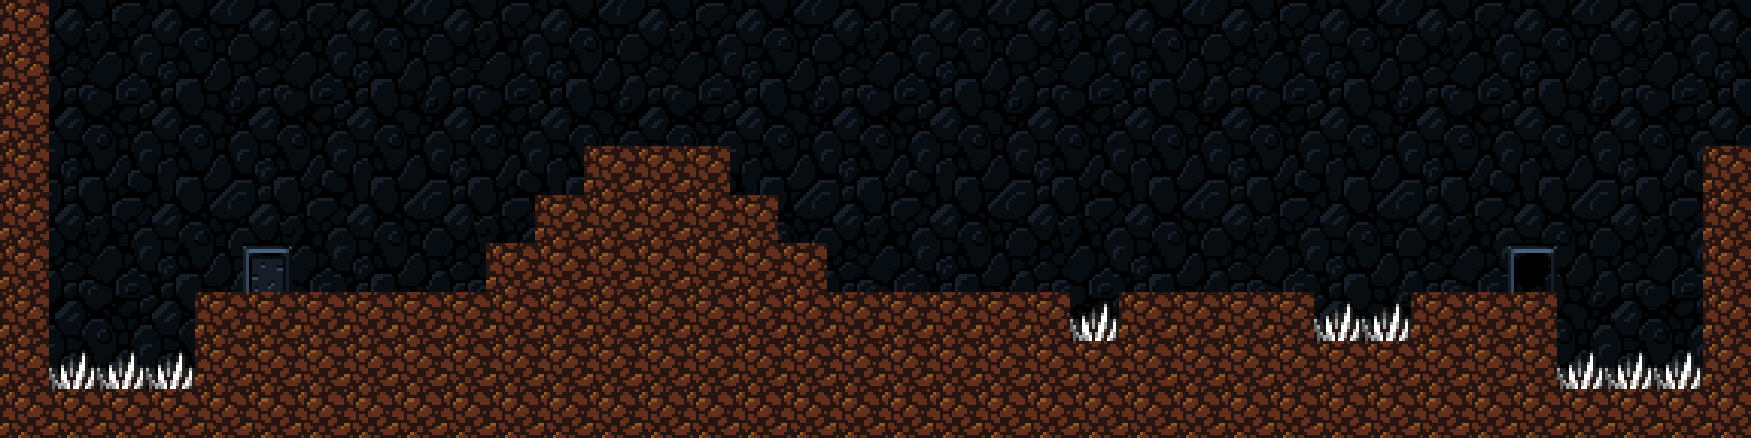
\includegraphics[width=\textwidth]{fig/levels/level1.pdf}
\caption{Cenário fácil, que explora o deslocamento horizontal do jogador.}
\label{fig:level1}
\end{figure}

O nível \textbf{médio}, além de explorar os elementos do nível \textit{fácil},
também requer que o jogador se desloque \textbf{verticalmente}. Esse nível é
mais difícil que o \textit{fácil} pois o jogador precisa \textbf{mudar de
direção} duas vezes. A figura \ref{fig:level2} mostra o nível médio, onde o
jogador deve se deslocar da entrada localizada na plataforma mais acima e à
esquerda até a saída que se encontra no canto direito e abaixo.

\begin{figure}[H]
\centering
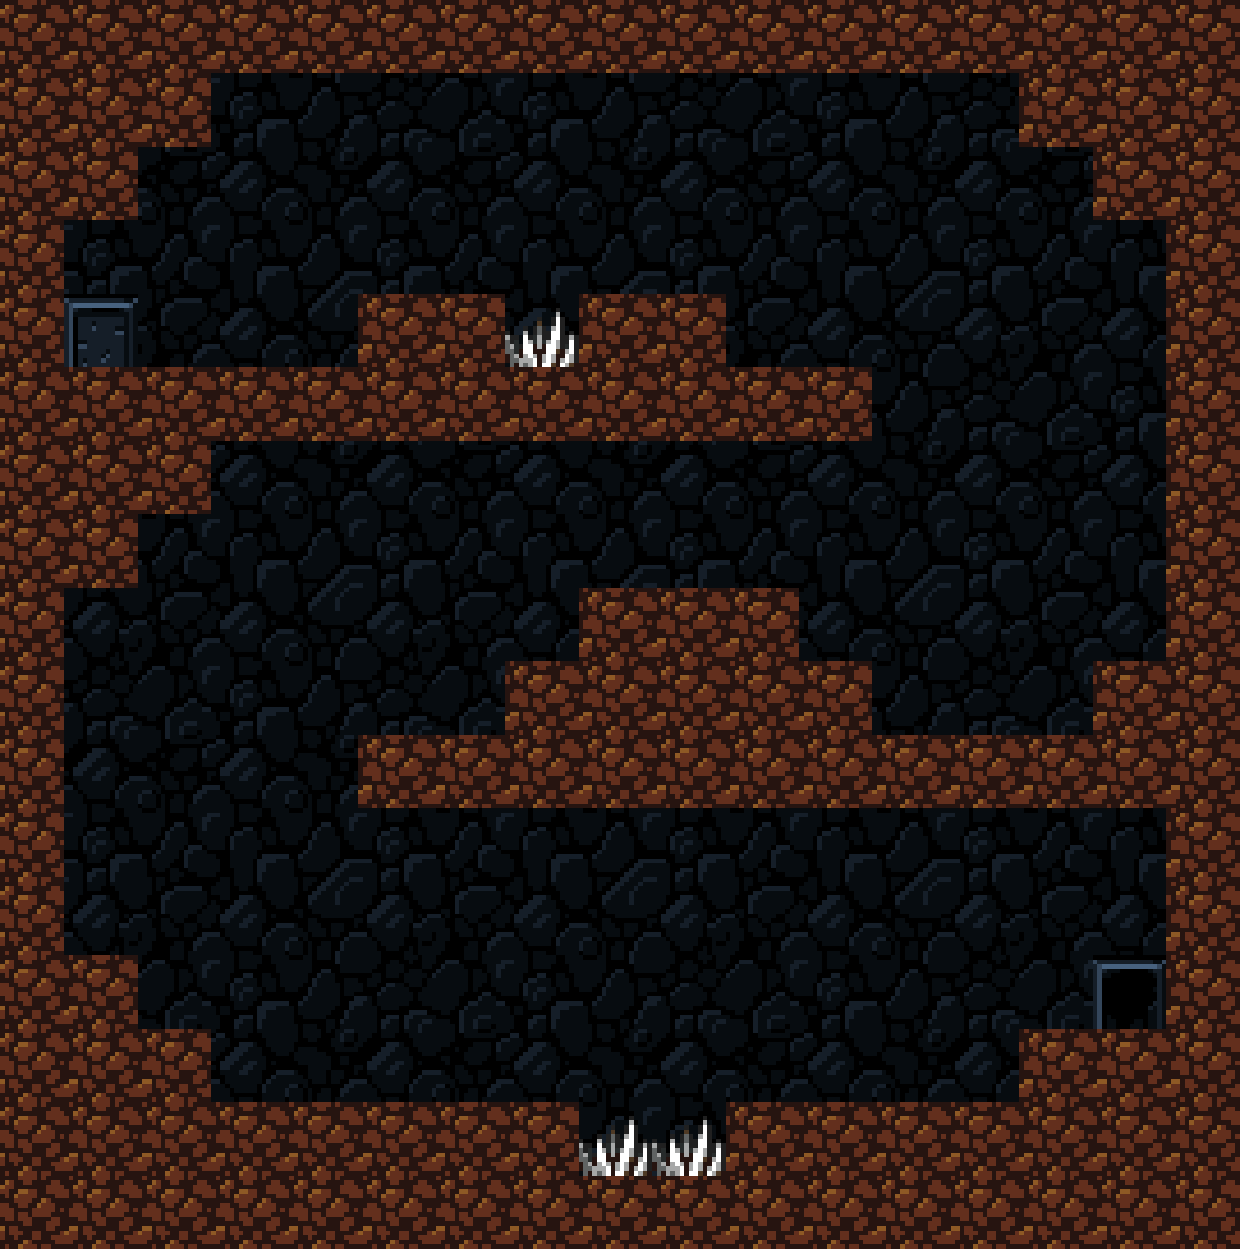
\includegraphics[width=\textwidth / 2]{fig/levels/level2.pdf}
\caption{Cenário médio, que explora o deslocamento horizontal e vertical do
    jogador, além de explorar a mudança de direção.}
\label{fig:level2}
\end{figure}

Para o nível médio, que conta com mais alguns desafios, estabelecemos os
seguintes \textbf{critérios de parada}:

\begin{description}
    \item [Número de execuções] no máximo \textbf{10000} execuções.
    \item [Tempo máximo de execução] no máximo \textbf{20 segundos} executando.
\end{description}

O nível \textbf{difícil} é um nível gerado aleatóriamente pelo jogo. Mesmo
sendo um nível gerado, é possível -- conforme a seção
\ref{section:spelunky-procgen-path} -- atravessar o nível sem a necessidade de
usar bombas, cordas ou outros equipamentos, sendo esse o desafio mais
interessante desse trabalho.

Por ser o cenário mais desafiador, estabelecemos os seguintes \textbf{critérios
de parada}:

\begin{description}
    \item [Número de execuções] no máximo \textbf{20000} execuções.
    \item [Tempo máximo de execução] no máximo \textbf{90 segundos} executando.
\end{description}

\section{Cenários Específicos}

Além dos desafios expostos nos níveis convencionais, existem alguns outros que
estão presentes em muitos níveis do jogo. Muitos deles requerem que alguns
botões sejam combinados ou pressionados em alguma sequência específica. Visando
explorar esses elementos, elaboramos alguns cenários para testes de situações
específicas.

Por serem cenários simplificados, elaboramos os seguintes \textbf{critérios de
parada} para todos eles:

\begin{description}
    \item [Número de execuções] no máximo \textbf{10000} execuções.
    \item [Tempo máximo de execução] no máximo \textbf{10 segundos} executando.
\end{description}

O cenário \textbf{extra 1}, exibido na figura \ref{fig:extra1}, conta com uma
escada que liga a plataforma inferior do jogo à plataforma superior. Portanto,
o jogador que deseja chegar até a porta de saída localizada na plataforma
superior deve fazer o uso dessa escada.

\begin{figure}[H]
\centering
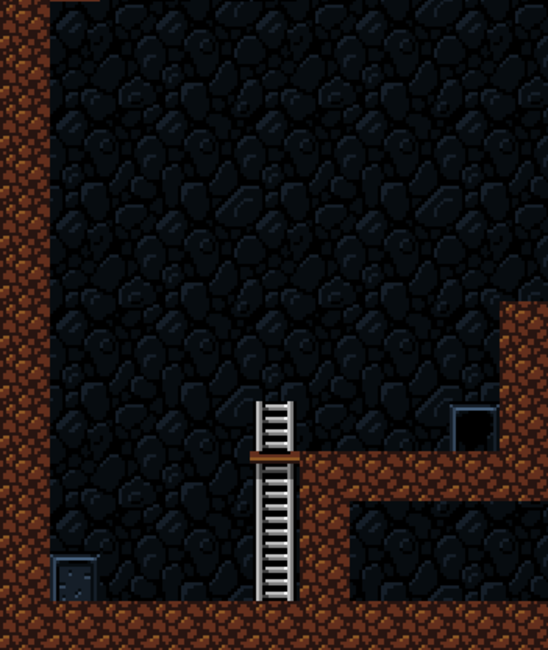
\includegraphics[width=\textwidth / 2]{fig/levels/extra1.pdf}
\caption{Cenário extra 1, que explora o uso de escadas por parte do jogador.}
\label{fig:extra1}
\end{figure}

Em alguns momentos, é necessário que o jogador se agarre à parede para poder
chegar até locais muito altos. Esse é um problema interessante, pois é
necessário a combinação das ações de movimentação e de salto. O nível
\textbf{extra 2} -- mostrado na figura \ref{fig:extra2} -- só pode ser vencido
caso o jogador salte, se agarre na parede e salte novamente, alcançando a
plataforma mais alta.

\begin{figure}[H]
\centering
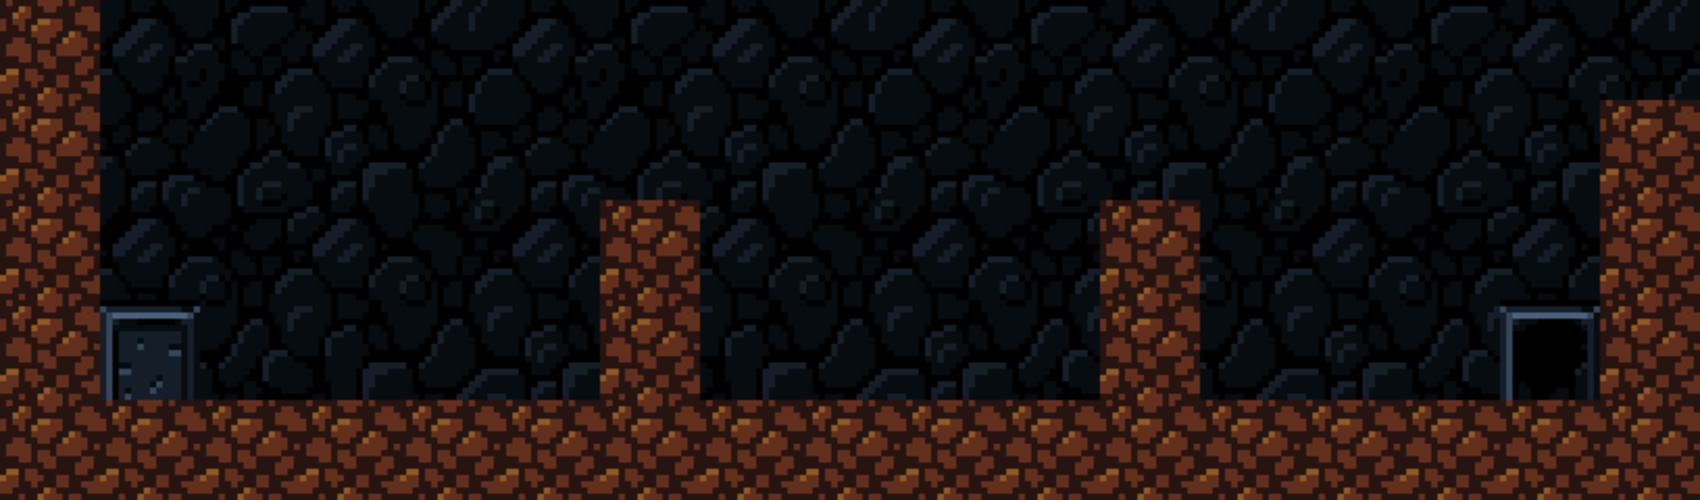
\includegraphics[width=\textwidth / 2]{fig/levels/extra2.pdf}
\caption{Cenário extra 2, que faz com que o jogador tenha que se agarrar à
    parede para vencer o nível.}
\label{fig:extra2}
\end{figure}

O jogo também conta com a possibilidade de \textbf{correr}, fazendo com que o
jogador se desloque mais rápido pelo nível. Além disso, quando o jogador corre,
é possível que este tenha uma impulsão maior no momento de saltar, podendo
passar por um número maior de obstáculos. De forma a explorar a corrida do
jogador, o nível \textbf{extra 3} -- representado na figura \ref{fig:extra3} --
só pode ser vencido se o jogador pular os espinhos enquanto estiver correndo.

\begin{figure}[H]
\centering
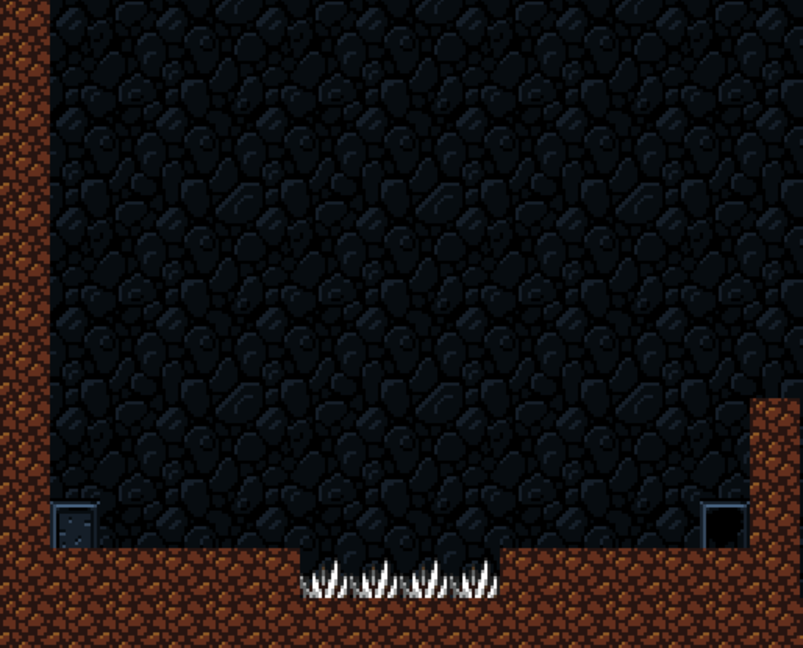
\includegraphics[width=\textwidth / 2]{fig/levels/extra3.pdf}
\caption{Cenário extra 3, que faz com que o jogador tenha que correr para
    vencer o nível.}
\label{fig:extra3}
\end{figure}

\todoin[caption={Cenários para Execução}] {
\begin{itemize}
	\item Mapas escolhidos:
	\begin{itemize}
		\item Easy (apenas alguns obstáculos)
		\item Medium (obstáculos e deslocamento vertical)
		\item Hard (mapa normal, gerado)
		\item Detalhar parâmetros de execução e critério de parada de cada mapa
	\end{itemize}

	\item Mapas adicionais (para teste de features):
	\begin{itemize}
		\item Motivação (tempo curto para explorar itens adicionais)
		\item Explorar corrida do bot
		\item Agarrando na parede
		\item Escadas
		\item Matar inimigos
		\item Coletar tesouros
		\item Detalhar parâmetros de execução e critério de parada de cada mapa
	\end{itemize}
\end{itemize}
}
